\documentclass[10pt]{article}
\usepackage{arxiv}
\usepackage[T1]{fontenc}
\usepackage{amsmath,amssymb,booktabs,graphicx,array,longtable}
\usepackage[hidelinks]{hyperref}
\renewcommand{\shorttitle}{NEUROGENESIS: Delayed-Credit Predictor Memory}
\renewcommand{\headeright}{Research Report}
\renewcommand{\undertitle}{A Reproducible Mechanism Study}
\title{NEUROGENESIS: Testing Bounded Predictor Memory\\under Delayed Feedback and Recurring Drift}
\author{Ryan Gomez}
\date{October 21, 2026}
\begin{document}
\maketitle
\begin{abstract}
Can retaining a small bank of frozen predictors replace some parameter updates in online regression without materially worsening prediction? We specify a delayed-credit predictor bank with prediction-time loss accounting, finite FIFO capacity, and an update-suppression gate. After two bounded development versions, a source-locked evaluation completes 1,260 attempts across 20 fresh seeds, seven conditions, and nine methods. On the five registered primary conditions, the candidate reduces paired relative mean squared error by 36.01\% against the development-selected RLS baseline (95\% bootstrap interval: 34.00--38.04\% reduction), while using 58.55\% fewer weight updates. All synthetic traces and checkpoints reproduce exactly in a clean virtual environment. However, six RLS-based methods, including candidate and baseline, fail numerically on chronological UCI Air Quality transfer, preventing a valid real-data comparison. The overall finding is mixed: the synthetic accuracy--update hypothesis is supported, but numerical robustness and real-data transfer remain unresolved. Expert reuse and update skipping are established ideas; no broad novelty or general-purpose model claim is made.
\end{abstract}
\keywords{online regression \and delayed feedback \and recurring concept drift \and bounded memory \and reproducibility}

\section{Introduction}
Online adaptation faces competing objectives. A predictor should incorporate newly available labels, but overwriting its parameters may remove a mapping that becomes relevant again. Delayed labels make this tension harder: the error that triggers an update can describe an environment that has already changed. A low error late in a stable interval therefore does not imply low error throughout an entire stream.

The NEUROGENESIS predecessor implemented a deterministic benchmark but no candidate mechanism. It evaluated frozen prediction, two SGD learning rates, and Adam on five development seeds. Its stronger-learning-rate SGD achieved very low late-regime error while suffering large transient errors. The predecessor's scientific scope was unresolved; none of its held-out identities was evaluated. We retain that result and introduce a successor rather than retroactively describing the baseline study as a successful memory method.

Our question is deliberately limited: can a finite bank of frozen linear predictors, selected using only legally available delayed losses, preserve accuracy within two percent of a development-selected conventional baseline while reducing weight updates by at least twenty percent? This is a falsifiable empirical question. It neither assumes that memory is beneficial nor promises a universal learning algorithm. We distinguish fewer weight updates from lower total arithmetic, runtime, or memory.

\section{Related work and novelty boundary}
Dynamic Weighted Majority already creates, weights, and removes experts according to performance \cite{dwm}. Delayed-feedback online learning has a general theoretical literature; the consequences of delay depend on the stochastic or adversarial setting \cite{delay}. Those results motivate explicit information timing but do not provide an off-the-shelf guarantee for our nonstationary gated predictor.

Conformal model reuse selects earlier models using tests of distributional relevance and performance \cite{conformal}. Continuous Evolution Pool uses forecaster retrieval, evolution, elimination, and gradient abandonment \cite{cep}. Dynamic Multi-period Experts combines period-specific experts, regression-based adaptation, and gating \cite{dyname}. Thus, neither an expert bank nor the combination of reuse and skipped updates constitutes a defensible broad novelty claim.

Our method uses small linear predictors and an exponentially weighted delayed-loss gate to make every decision traceable. The experiment targets information timing, bounded capacity, and update accounting. We do not reproduce the full neural forecasting systems in CEP or DynaME, and make no superiority claim over them. The reference controls answer a narrower mechanism question on the declared tasks.

\section{Problem formulation}
At step $t$ a feature vector $x_t\in\mathbb R^d$ arrives. Write $\tilde x_t=(x_t^\top,1)^\top$ and $p=d+1$. The learner predicts $\hat y_t$ before observing $y_t$. Feedback is delivered at $a_t=t+D$. Before prediction at $t$, the runner may deliver labels $y_s$ only when $s<t$ and $a_s\leq t$. With zero delay, the current label is delivered after its prediction. The runner scores errors externally; a learner never receives regime annotations or unreleased targets.

The primary loss is prequential squared error:
\[
 \operatorname{MSE}=\frac{1}{|\mathcal O|}
 \sum_{t\in\mathcal O}(\hat y_t-y_t)^2,
\]
where $\mathcal O$ contains observations with a present target. Missing targets remain on the clock but do not enter the loss or update stream. State is reset between independent synthetic tasks. For chronological real transfer, legal warmup state continues into the test interval.

\section{Method}
\begin{figure}[ht]\centering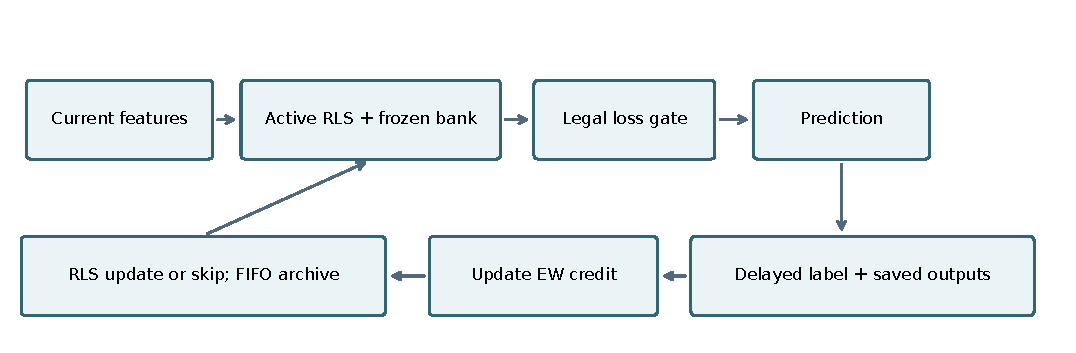
\includegraphics[width=\linewidth]{figures/architecture.pdf}\caption{Prediction and feedback flow. Delayed credit uses saved prediction-time outputs; adaptation uses the current active state.}\end{figure}

\subsection{State and initialization}
The active predictor is $w_t\in\mathbb R^p$, initialized to zero, with RLS covariance $P_0=10I$. A FIFO bank contains at most $K$ frozen vectors $v_j$, unique increasing integer IDs, observed-loss estimates $L_j$, and feedback counts $n_j$. The active predictor has its own estimate $L_0$ and count. The bank starts empty. A prediction ticket stores the active output and each currently existing expert's output; the runner retains the ticket with the example until its label is delivered.

\subsection{Prediction and delayed credit}
Every prediction computes $p_{t,0}=w_t^\top\tilde x_t$ and $p_{t,j}=v_j^\top\tilde x_t$. Eligible experts satisfy
\[
 n_j\geq m,\qquad L_j<gL_0,\qquad L_j\leq h.
\]
Among them, choose the smallest loss, breaking ties by the smallest ID. With no eligible expert, use the active predictor. The uniform-bank ablation averages all bank outputs and the active output.

When $y_s$ becomes available, update the loss of every surviving expert that actually predicted example $s$:
\[
 L_j\leftarrow
 \begin{cases}
 (p_{s,j}-y_s)^2,&n_j=0,\\
 (1-\alpha)L_j+\alpha(p_{s,j}-y_s)^2,&n_j>0.
 \end{cases}
\]
Then increment $n_j$. The active loss is updated analogously using its cached output. An expert born after step $s$ receives no score for $s$. An evicted expert's ticket entry is ignored; IDs are never recycled. This prevents accidental credit assignment to a different expert.

\subsection{Update suppression and adaptation}
After processing the new losses, re-evaluate the gate. If an archived expert qualifies and suppression is enabled, skip the active parameter update. Otherwise apply forgetting-factor recursive least squares:
\[
 \begin{aligned}
 q&=P\tilde x_s, &z&=\lambda+\tilde x_s^\top q, &\lambda&=0.95,\\
 w&\leftarrow w+q(y_s-w^\top\tilde x_s)/z,
 &P&\leftarrow(P-qq^\top/z)/\lambda.
 \end{aligned}
\]
The residual uses current weights on an available example. It is not the stale prediction-time residual. Tickets are used for prospective credit; current residuals are used for adaptation. Every $S$ actual active updates, append a frozen copy of $w$, assigning a new ID. If this exceeds capacity, evict the oldest bank member.

The all-update ablation has the same prediction rule, bank capacity, and scoring mechanism but never suppresses the active update. Its bank trajectory can consequently differ; this is part of the intervention's downstream effect. The no-bank ablation is ordinary RLS with the same forgetting factor. When an update is skipped, both weights and covariance remain unchanged; no hidden covariance update is performed.

For the sequence of accepted update examples indexed by $i=1,\ldots,n$, this RLS recursion corresponds to the regularized exponentially weighted objective
\[
 \min_w\ \sum_{i=1}^{n}\lambda^{n-i}(y_i-w^\top\tilde x_i)^2
 +\frac{\lambda^n}{10}\|w\|^2.
\]
The initialization $P_0=10I$ supplies the inverse ridge precision. Suppression therefore changes the accepted-example sequence and the forgetting clock, in addition to the update count. It does not preserve the same wall-clock weighting as always-updating RLS. The comparison tests this full intervention; it cannot isolate a claim about memory capacity alone.

\subsection{Mathematical property and limits}
For the NLMS control, one available example with residual $e=y-w^\top\tilde x$ and $q=\|\tilde x\|^2$, the NLMS step produces
\[
 e'=e\left(1-\eta\frac{q}{\epsilon+q}\right).
\]
For $0<\eta<2$, the same-example residual magnitude cannot increase. This follows by substituting the update into $y-w'^\top\tilde x$; it is checked against hand-computable examples in the unit suite. It is not a theorem about future risk, expert selection, or drifting environments.

The NLMS control uses $\epsilon=10^{-8}$ and updates the augmented intercept as another coordinate. For RLS, the denominator $z$ must stay positive; a nonpositive value, nonfinite covariance, nonfinite output, or state-budget violation creates a retained failed attempt rather than a seed retry. All vector and covariance dimensions are explicit in the checkpoint.

With identical feature distributions under two different hidden target mappings, a policy has no label evidence to identify an unannounced switch until informative feedback arrives. Memory cannot remove that information limitation. Moreover, an archived predictor may be obsolete, FIFO eviction may remove a useful concept, and skipping active updates may prevent acquisition of a new regime.

\subsection{Complexity and resource accounting}
Prediction requires $O(Kp)$ arithmetic. Pending tickets add $O(D(p+K))$ state; bank vectors use $O(Kp)$ state and the active covariance uses $O(p^2)$ state. Available-label credit requires $O(K)$ scoring work, with an additional $O(p^2)$ active RLS update when admitted. We count gradients, updates, dot products, estimated coordinate arithmetic, bank writes, example-cache writes, evictions, predictions routed to memory, and skipped updates. Counts describe the reference implementation; sorting, Python allocation, and interpreter overhead are reflected in wall time and process RSS, not a claim of exact hardware FLOPs.

The common numerical-state ceiling is 128 KiB per attempt. Numerical state is distinct from Python object memory, retained output traces, and compressed checkpoint size. Process peak RSS is recorded with a 512 MiB ceiling. Equal ceilings do not imply identical actual resources; efficiency claims must use measured usage.

Reported attempt wall time includes result/checkpoint serialization. Process peak RSS is the process high-water mark, not an isolated incremental allocation attributed to one method. Timing on a shared host is descriptive and is not evidence of a hardware-independent speedup.

\section{Experimental methodology}
\subsection{Synthetic data and independent units}
The successor contains eight regimes with normalized four-dimensional linear target maps embedded in eight observed features. Remaining coordinates are distractors. Base streams contain 960 predictions, noise standard deviation $0.05$, and delay four. Maps are generated from a seeded Gaussian vector and normalized; the second map negates the first. The recurring sequence is $[0,1,0,2,1,0,2,0]$. Odd-numbered regimes increase distractor standard deviation to three. A no-recurrence condition uses eight distinct maps.

Five primary conditions are base recurrence, delay 16, noise $0.2$, distractor scale six in shifted regimes, and 16 observed dimensions. Secondary conditions are no recurrence and a 1,920-step horizon. Policies do not receive those labels. Development uses seeds 1201, 1213, 1223, 1237, and 1249 on base and no-recurrence streams. Confirmation uses 20 fresh seeds, 90001--90020, across all seven conditions. The independent unit is a seed, not a time step; conditions sharing a seed are grouped before uncertainty estimation.

\subsection{Search budget and controls}
The final candidate grid contains exactly eight choices: $h\in\{0.02,0.1\}$, $\alpha\in\{0.2,0.5\}$, and $K\in\{4,8\}$. Fixed values are $S=32$, $m=8$, and $g=0.9$. Select the minimum mean development MSE over both conditions and all five seeds, with lexicographic name tie-breaking.

The conventional grid includes NLMS learning rates $0.1,0.5,1.0$; Adam learning rates $0.001,0.01,0.05$; RLS forgetting factors $0.95,0.99,1.0$; frozen zero prediction; last-observation prediction; a 32-example FIFO three-nearest-neighbor regressor; and FIFO replay NLMS. Adam uses current residuals, $\beta_1=0.9$, $\beta_2=0.999$, $\epsilon=10^{-8}$, and gradient norm limit ten. RLS starts with covariance $10I$. Replay applies one extra update to the oldest stored example per new available label. Selection of the conventional comparator uses the same development endpoint and full denominator.

Confirmation includes the selected candidate and baseline, all-update bank, capacity-one bank, uniform-bank prediction, no-bank RLS, replay, nearest-neighbor cache, and frozen prediction. Each development grid contains 210 attempts; confirmation contains 1,260. Both development matrices and all final confirmatory attempts completed; execution receipts and full raw traces are retained. The selected v3 configuration is $h=0.1$, $\alpha=0.5$, $K=8$, and $\lambda=0.95$.

\subsection{Statistical decision rule}
For seed $s$, average MSE over the five primary conditions separately for candidate and comparator, then compute the relative difference
\[
 \Delta_s=\frac{\overline{\operatorname{MSE}}_{\mathrm{candidate},s}}
 {\overline{\operatorname{MSE}}_{\mathrm{baseline},s}}-1.
\]
Use 10,000 paired seed bootstrap resamples with fixed analysis seed 20261021. The predeclared hypothesis is supported only if the upper 95\% interval bound is at most $0.02$, average update reduction is at least $0.20$, and every primary cell is valid and complete. Accuracy superiority is separately defined by an upper bound below $-0.05$. Missing or failed cells prevent a support declaration. Secondary comparisons are descriptive, with no multiplicity-unadjusted family of significance claims.

If the lower interval exceeds the noninferiority margin, or the measured mean update reduction is below its threshold, the predefined joint claim is negative. Otherwise a non-supporting uncertain result is inconclusive. An invalid experiment is a different state. Neither permits pretending the method succeeded. Confirmatory outcomes cannot be used to revise the tested candidate.

\subsection{Real temporal transfer}
The UCI Air Quality dataset records hourly sensor responses and gas reference measurements \cite{uci}. The downloaded CSV contains 9,357 nonblank timestamped rows from March 10, 2004 through April 4, 2005; this differs from the landing page's summarized count and date range. We retain the file checksum and actual timestamps.

The target is CO(GT), divided by ten. Inputs are five metal-oxide sensor channels, temperature, relative humidity, and absolute humidity. Other reference gas concentrations are excluded. Fixed scales are 1000 for sensor channels, 50 for temperature, 100 for relative humidity, and two for absolute humidity. Each missing feature, encoded as $-200$, is replaced by zero and accompanied by a missingness indicator, giving 16 input coordinates. This uses no full-stream fitted normalization.

The first 40\% of rows provide chronological warmup; the final 60\% form protected transfer, with state carried forward legally. Settings are selected on synthetic development only. An artificial four-hour label delay is imposed; actual label-release timestamps are not available. Missing target rows remain in sequence and receive predictions but are not scored or trained upon. We report original-unit MSE by multiplying scaled MSE by 100. Seven contiguous blocks are descriptive summaries, not seven independent datasets.

\subsection{Bounded development revision}
The first successor (v2) used NLMS snapshots and a relative-only gate. Its best development MSE was 0.80245, compared with 0.33732 for RLS. This motivated one recorded successor (v3): RLS forms the snapshots, and an absolute loss ceiling prevents selecting a merely less inaccurate stored expert. Both changes are declared together; their individual effects are not identified by the main experiment. No protected outcomes were inspected before this revision. The two-version development budget is exhausted, and no further outcome-driven model changes are admitted.

\section{Results and evidence disposition}
\subsection{Frozen synthetic evaluation}

The completed matrix contains 1,260 attempts and no failed cells. The predefined synthetic disposition is \textbf{SUPPORTED}. Across the primary conditions, the mean paired seed-level relative MSE change is -36.01\% (95\% bootstrap interval [-38.04, -34.00]\%). Mean weight-update reduction is 58.55\%. These quantities use the frozen aggregation rule; the table below reports pooled means over the same balanced conditions.

\begin{table}[ht]\centering\small\begin{tabular}{lrrrr}\toprule Method & MSE & Updates & Arithmetic & State bytes\\\midrule

Always-update bank & 0.4445 & 953.6 & 974385 & 5456 \\

RLS baseline & 0.5378 & 953.6 & 798925 & 3280 \\

Memory gate & 0.3426 & 395.2 & 499856 & 5456 \\

Capacity 1 & 0.5411 & 875.4 & 758486 & 3504 \\

Frozen zero & 1.0097 & 0.0 & 26074 & 1992 \\

FIFO kNN & 0.9124 & 0.0 & 981053 & 5576 \\

No bank (RLS) & 0.5378 & 953.6 & 798925 & 3280 \\

FIFO replay & 1.0540 & 1906.2 & 173286 & 5576 \\

Uniform bank & 1.0036 & 395.2 & 499856 & 5456 \\

\bottomrule\end{tabular}\caption{Primary-condition means over 100 task instances per method. State is maximum numerical state, not process RSS.}\end{table}

\begin{figure}[ht]\centering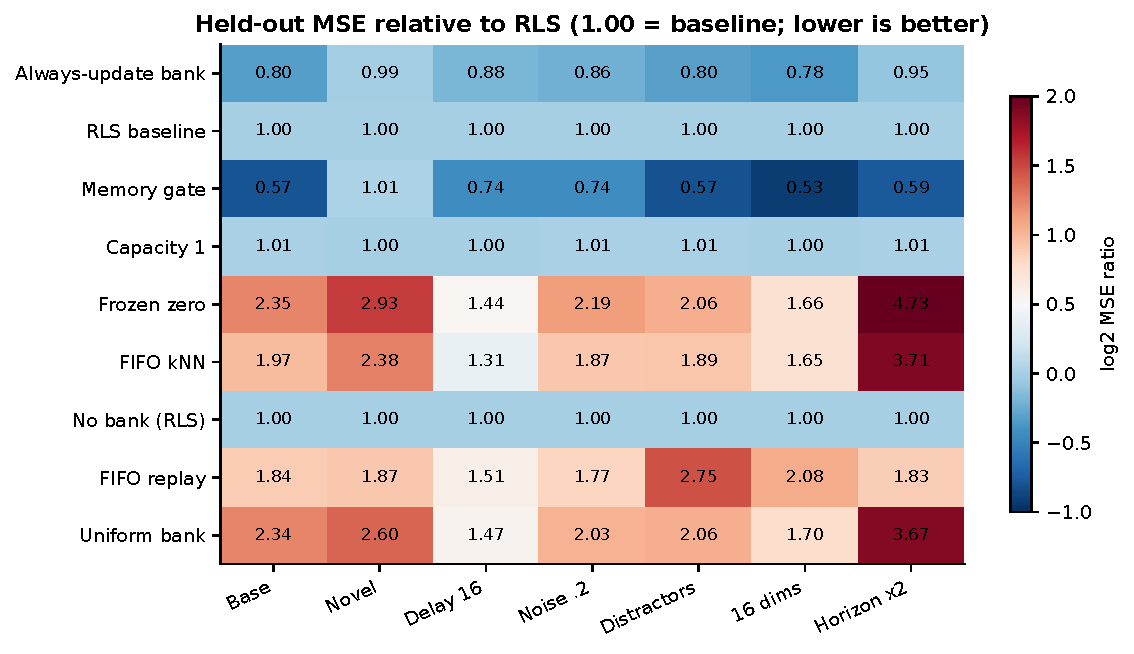
\includegraphics[width=\linewidth]{figures/condition_heatmap.pdf}\caption{Complete condition matrix. Values are mean-MSE ratios, not paired-effect confidence bounds.}\end{figure}

\begin{figure}[ht]\centering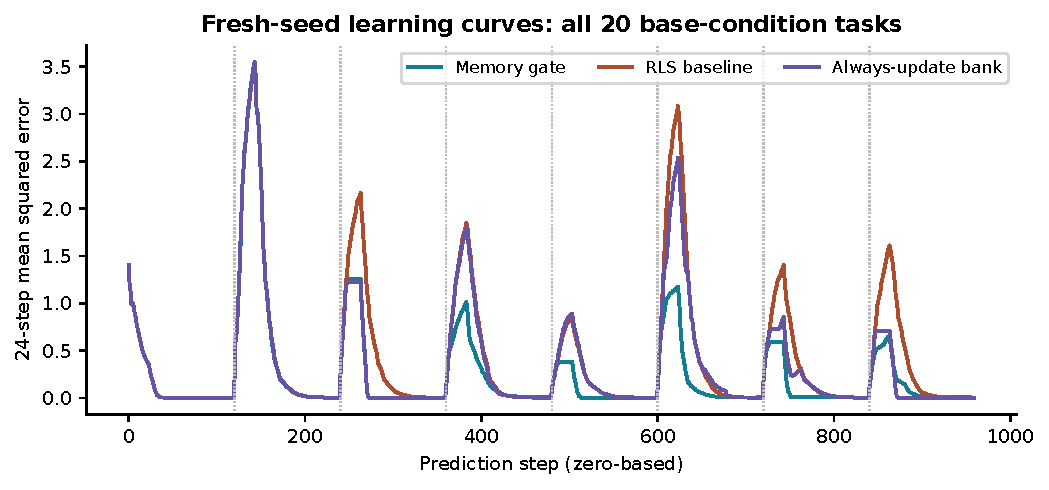
\includegraphics[width=\linewidth]{figures/learning_curves.pdf}\caption{Rolling errors averaged over all 20 fresh base-condition seeds. Vertical lines mark generator changes, hidden from the learner.}\end{figure}

Against the all-update bank, the candidate relative MSE change is -22.66\% (95\% interval [-24.65, -20.73]\%). This comparison is descriptive mechanism evidence and is distinct from the primary baseline test.

\begin{figure}[ht]\centering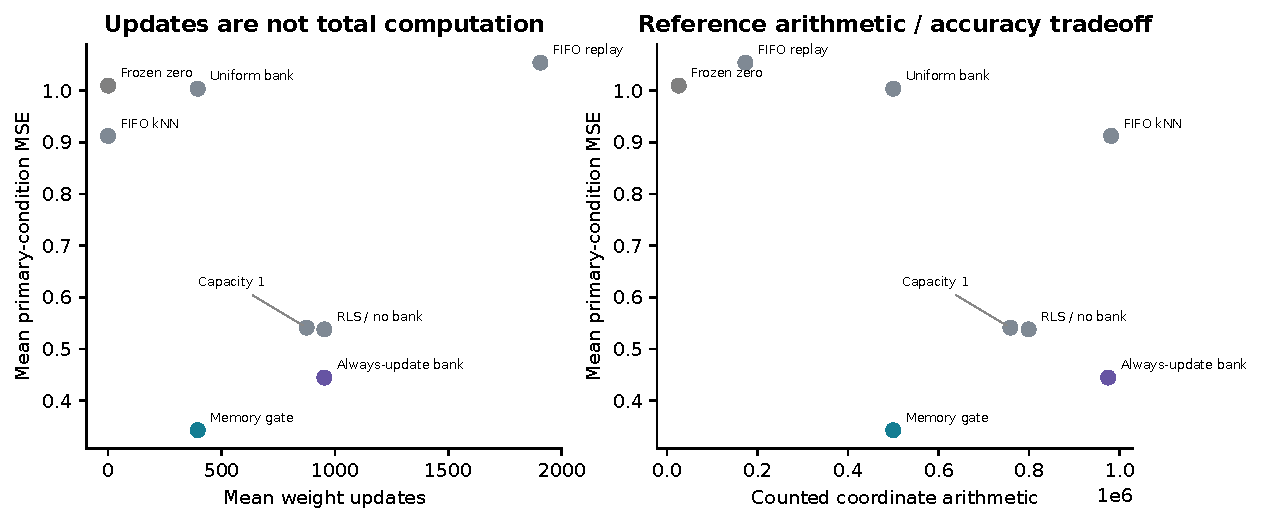
\includegraphics[width=\linewidth]{figures/efficiency.pdf}\caption{Accuracy versus actual update counts and counted arithmetic. Additional prediction work can offset gradient savings.}\end{figure}

\subsection{Chronological real-data transfer}

All ten registered methods were attempted. Six RLS-based methods failed because the covariance update lost positive definiteness: the candidate, baseline, all-update bank, capacity-one bank, uniform bank, and no-bank RLS. The candidate failed after 6,702 predictions; the baseline failed after 710, before the test boundary. Their partial errors are not substitutes for a full-transfer comparison. Four controls completed, each scoring 4,668 test targets. Real-transfer efficacy is therefore \textbf{not established}. The overall evidence disposition is \textbf{MIXED}: supported on the registered synthetic endpoint, with a numerical failure preventing the real-data comparison.

\begin{table}[ht]\centering\small\begin{tabular}{lrr}\toprule Method & CO MSE & Test updates\\\midrule

Always-update bank & FAILED & --- \\

RLS baseline & FAILED & --- \\

Memory gate & FAILED & --- \\

Capacity 1 & FAILED & --- \\

Frozen zero & 7.606414 & 0 \\

FIFO kNN & 0.913742 & 0 \\

Last observation & 3.228987 & 0 \\

No bank (RLS) & FAILED & --- \\

FIFO replay & 0.551697 & 9336 \\

Uniform bank & FAILED & --- \\

\bottomrule\end{tabular}\caption{All real-transfer methods, including a last-observation control.}\end{table}

\begin{figure}[ht]\centering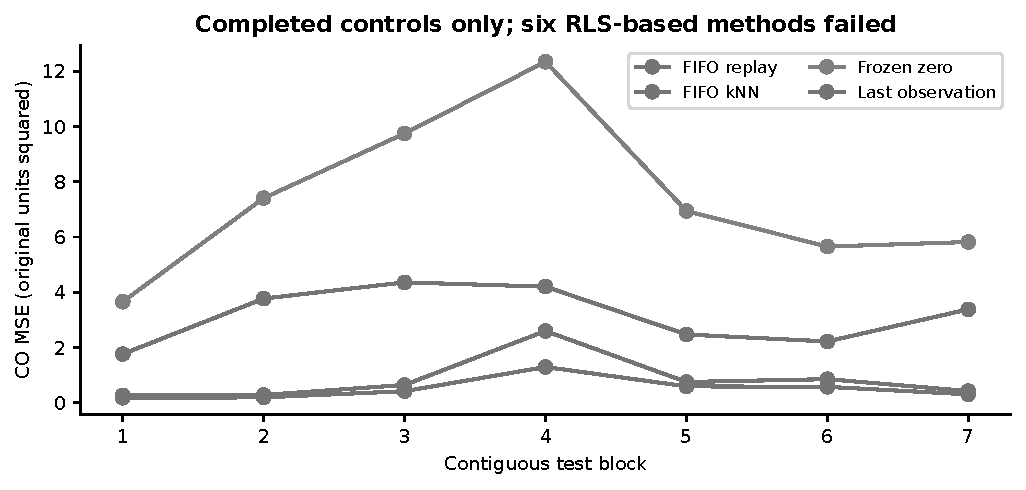
\includegraphics[width=\linewidth]{figures/real_transfer.pdf}\caption{Seven contiguous temporal blocks are descriptive, not independent replications.}\end{figure}

\subsection{Evidence boundary}

These are executed local CPU results. Kaggle execution and independent external replication are separate release gates; this manuscript does not infer them from the presence of a notebook or package. The v1 protected evaluation remains untouched.

\subsection{Interpretation of controls and costs}
The no-recurrence condition gives pooled MSE 0.3444 for the candidate and 0.3394 for RLS (1.48\% higher), so the improvement does not extend to every registered condition. Capacity one and uniform averaging do not reproduce the primary accuracy benefit. Baseline and no-bank predictions coincide because both instantiate the selected RLS configuration; they are not separate independent replications.

On the primary conditions, the candidate uses 37.43\% fewer counted coordinate operations than RLS, but maximum numerical state is 5456 versus 3280 bytes. Mean recorded attempt time is 0.3959 versus 0.3958 seconds, including serialization on a shared host. Thus the recorded timing does not establish a speed advantage despite fewer active updates and counted operations.


\section{Failure analysis}
Three failure classes must remain separate. A numerical or protocol defect can invalidate an experiment and requires a documented correction. A valid but unfavorable result rejects or limits the hypothesis. A resource or platform refusal produces no scientific outcome at all.

The executed real-transfer failures expose a limitation of covariance-form RLS under extreme conditioning. At failure, covariance matrices are symmetric but have negative minimum eigenvalues, with maximum eigenvalues between approximately $10^{15}$ and $10^{29}$. A vanishing ridge penalty and correlated missingness indicators can produce large unobserved-direction uncertainty. Small-system mathematical agreement therefore does not guarantee reliable long-stream floating-point behavior. Symmetrizing the covariance alone cannot resolve this observed failure. The frozen candidate is preserved; a post-outcome numerical diagnostic cannot replace its registered outcomes. A post-outcome square-root information QR diagnostic matched batch ridge in 30 small systems and completed the stream, but the control produced catastrophic error (approximately $2.45\times10^{62}$) and coefficients of magnitude $10^{47}$. The candidate also retained coefficients above $10^8$. Thus an exception-free representation is not an adequate robustness repair. These diagnostic outcomes are excluded from the main efficacy tables; persistent regularization or rank handling would change the statistical model and require a separately frozen successor.

The predecessor establishes a relevant warning: choosing a model by its last few iterations can hide severe accumulated error. The successor therefore scores the entire prediction stream, retains every seed, and reports cost alongside accuracy. A strong RLS or NLMS result would be evidence against the need for this memory gate on these tasks, rather than a reason to remove that baseline.

When the gate reuses a historical model, it may save parameter updates but still perform more dot products than a single predictor. If an apparent improvement disappears against the all-update bank, the evidence does not identify suppression as the cause of an accuracy advantage. If a benefit appears only in a post-hoc subgroup, that subgroup is exploratory and requires a separately frozen successor.

\section{Engineering verification and reproducibility}
The implementation is standard-library Python. Tests cover an exact NLMS contraction identity, scalar RLS agreement with ridge regression, delay-zero and delayed-label ordering, future-target poisoning, unavailable expert credit, FIFO identity, gate eligibility, missing-label clocks, finite-value rejection, complete method resets, and exact checkpoint restoration across eight method families.

Each attempt records source/config/task identity, raw prediction trace, counters, final full checkpoint, wall time, RSS, and success or failure. Gzip metadata is fixed to support deterministic compressed artifacts. Output directories cannot be overwritten. Freeze selection is recomputed from verified attempt results and binds source, protocol, dataset manifest, and development artifacts.

An additional independent mathematical check solves the batch exponentially weighted ridge normal equations by pivoted Gaussian elimination and compares them with RLS for 60 combinations of seed, forgetting factor, and accepted-update sequence. This checks the multivariate recursion and the skipped-update clock.

The main verifier recomputes metrics and can replay the model exactly. A separate auditor checks arithmetic and feedback legality without importing model or metric implementations. Its supplementary version permits relative $10^{-12}$ and absolute $10^{-15}$ tolerance when comparing a streaming sum with the main implementation's accurately accumulated mean; the frozen exact-equality auditor's rounding rejection is retained. This verifier correction does not change any result, model, or decision threshold. These are complementary code paths controlled by the same project. They are not independent external replication or peer review.

The Kaggle notebook embeds a hash-checked source/data archive and executes tests, the already frozen confirmation, analysis, real transfer, and verification. A saved output archive is required to claim hosted execution. An uploaded notebook or running editor is not a completed experiment.

\section{Discussion and limitations}
This study can establish only a bounded claim on synthetic linear regression and one temporal sensor stream. It does not establish efficacy for deep networks, learned objectives, causal reasoning, general intelligence, real-time deployments, or every distribution shift. The candidate consists of known components and a specific gate, so any methodological novelty remains limited.

The protected synthetic seeds test fresh realizations of declared generators, not arbitrary real-world generalization. The real stream is a single correlated sequence with artificial delay and an imperfect historical dataset description. The fixed scaling is intentionally simple. Full comparisons to recent neural forecaster-pool systems remain outside the executed control set.

Fewer active updates are not automatically lower compute or energy. Python timings reflect the reference implementation and the particular execution environment. Bootstrap intervals over 20 seeds have finite precision and do not repair limited task diversity. A negative result may still be informative if it identifies when a simple baseline removes the apparent need for a mechanism.

\section{Conclusion}
The frozen predictor-memory candidate satisfies the registered synthetic hypothesis: 36.01\% lower paired relative error and 58.55\% fewer weight updates than the selected RLS baseline. It also improves error over the all-update bank on the primary conditions, but does not improve every tested setting. Covariance failures prevent a valid real-transfer comparison. The defensible overall disposition is MIXED, with a supported synthetic claim and unresolved numerical robustness outside that setting. The result motivates separately qualified numerical work and genuinely unexposed external validation; it does not justify a perfect-model, universal-transfer, or state-of-the-art claim.

\appendix
\section{Implementation correspondence}
\begin{tabular}{p{.30\linewidth}p{.63\linewidth}}
\toprule
Scientific component & Executable implementation\\
\midrule
Prediction and expert eligibility & \texttt{engine.Policy.predict}, \texttt{winner}\\
Delayed prediction-time credit & \texttt{engine.Policy.observe}, ticket expert IDs\\
RLS and archival updates & \texttt{engine.Policy.rls}, \texttt{observe}\\
Label-release boundary & \texttt{engine.Runner.deliver}, \texttt{advance}\\
Exact restoration & \texttt{engine.Runner.restore}, \texttt{Policy.restore}\\
Selection and source lock & \texttt{experiment.freeze}, \texttt{source\_map}\\
Paired analysis & \texttt{experiment.analyze}, \texttt{bootstrap}\\
Real-data clock and transformation & \texttt{real\_transfer.load\_data}\\
Separate arithmetic audit & \texttt{audit.audit}\\
\bottomrule
\end{tabular}

\section{Algorithm chronology}
For every step, deliver past labels whose availability has arrived; predict the current example with active and archived experts; choose the eligible expert or active output; score outside the policy; store the pending ticket; then deliver any zero-delay current feedback. For every delivered label, score only experts that predicted it, re-evaluate the gate, update or skip active weights, and archive at the registered update interval. No step uses a future target or oracle regime label.

\section{Reproduction commands}
From \texttt{successors/memory\_v3}, run the following with fresh output paths:
\begin{verbatim}
python3 -m unittest discover -s . -p 'test_*.py' -v
python3 experiment.py develop --output runs/development
python3 experiment.py verify --input runs/development \
  --output runs/development-verification.json --replay
python3 experiment.py freeze --input runs/development \
  --output runs/freeze.json
python3 experiment.py confirm --lock runs/freeze.json \
  --output runs/confirmation
python3 experiment.py analyze --input runs/confirmation \
  --lock runs/freeze.json --output runs/analysis.json
python3 real_transfer.py run --lock runs/freeze.json \
  --output runs/real-transfer
python3 publication/audit_arithmetic.py \
  runs/confirmation runs/audit.json
python3 publication/verify_real_outcome.py \
  --input runs/real-transfer --output runs/real-audit.json
\end{verbatim}
Exact verification replay is permitted; a fresh hypothesis cannot reuse exposed confirmation outcomes as protected evidence. Local execution additionally checks a 512 MiB resource reserve and non-rising pageouts before phase admission.

\section{Authorship, licensing and ethics}
The report names Ryan Gomez, subject to owner verification before external submission. Implementation and drafting used AI assistance; this does not constitute independent scientific review. No new human-subject data were collected. UCI supplies public environmental measurements. Its landing page shows CC BY 4.0 and a legacy research-only notice; this artifact is for noncommercial research and retains attribution. The local refined \texttt{arxiv.sty} is copied with its checksum and provenance. No affiliation, venue acceptance, arXiv endorsement, or external reproduction is claimed.

\begin{thebibliography}{9}
\bibitem{dwm} J. Z. Kolter and M. A. Maloof. Dynamic Weighted Majority: An Ensemble Method for Drifting Concepts. \emph{JMLR}, 8:2755--2790, 2007. \url{https://www.jmlr.org/papers/v8/kolter07a.html}.
\bibitem{delay} P. Joulani, A. Gyorgy, and C. Szepesvari. Online Learning under Delayed Feedback. \emph{ICML, PMLR} 28(3):1453--1461, 2013. \url{https://proceedings.mlr.press/v28/joulani13.html}.
\bibitem{conformal} C. Eliades and H. Papadopoulos. A Conformal Martingales Approach for Recurrent Concept Drift. \emph{COPA, PMLR} 266:706--724, 2025. \url{https://proceedings.mlr.press/v266/eliades25a.html}.
\bibitem{cep} T. Zhan, M. Jin, Y. He, Y. Liang, and S. Pan. Continuous Evolution Pool: Taming Recurring Concept Drift in Online Time Series Forecasting. arXiv:2506.14790v3, 2026 revision. \url{https://arxiv.org/abs/2506.14790}.
\bibitem{dyname} S. Hong, S. Chae, S. Kim, S. Jang, and H. Yu. Dynamic Multi-period Experts for Online Time Series Forecasting. \emph{The ACM Web Conference}, 2026. doi:10.1145/3774904.3792731. \url{https://arxiv.org/abs/2603.09062}.
\bibitem{uci} S. De Vito et al. Air Quality. \emph{UCI Machine Learning Repository}. \url{https://archive.ics.uci.edu/dataset/360/air+quality}. Associated study: On field calibration of an electronic nose for benzene estimation in an urban pollution monitoring scenario. \emph{Sensors and Actuators B}, 129(2), 2008.
\end{thebibliography}
\end{document}
